\begin{figure}[htbp]
\section*{ WWOX}
\centering
\begin{subfigure}[b]{0.95\textwidth}
\centering
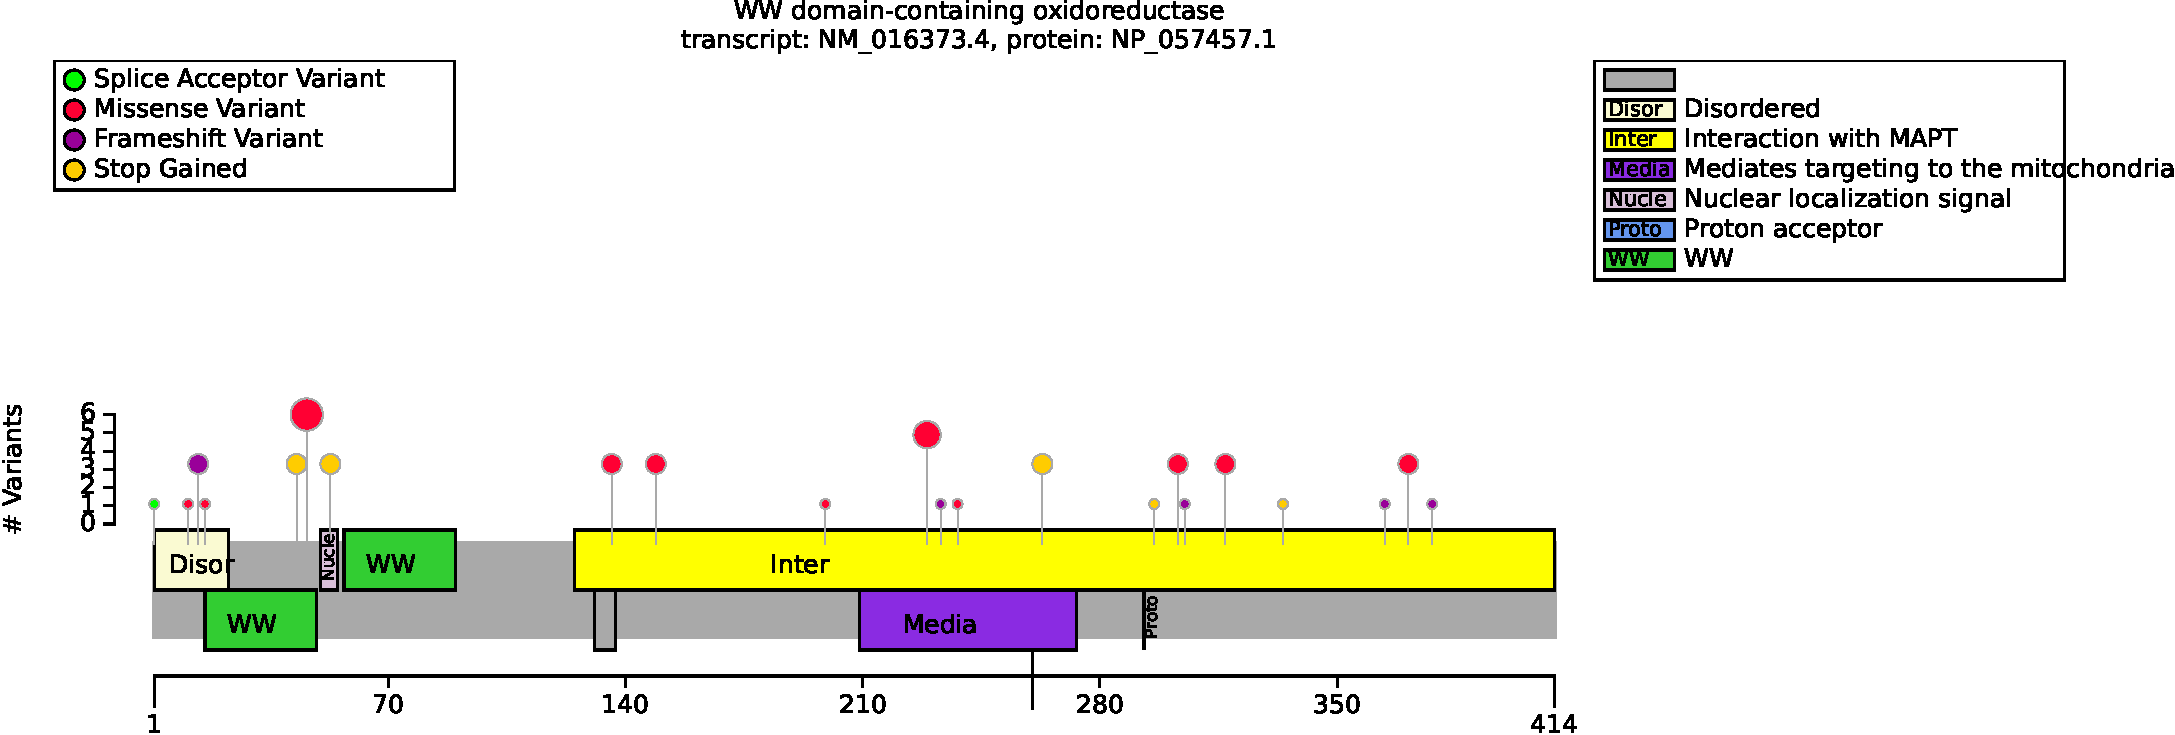
\includegraphics[width=\textwidth]{ img/WWOX_protein_diagram.pdf} 
\captionsetup{justification=raggedright,singlelinecheck=false}
\caption{Distribution of variants in WWOX}
\end{subfigure}

\vspace{2em}

\begin{subfigure}[b]{0.95\textwidth}
\centering
\resizebox{\textwidth}{!}{
\begin{tabular}{llllrr}
\toprule
HPO term & MAPT Interaction/MAPT Interaction OR MAPT Interaction/Other & Other/Other & p-value & adj. p-value\\
\midrule
Bilateral tonic-clonic seizure with focal onset [HP:0007334] & 0/18 (0\%) & 7/9 (78\%) & $4.05\times 10^{-5}$ & 0.002\\
\bottomrule
\end{tabular}
}
\captionsetup{justification=raggedright,singlelinecheck=false}
\caption{Fisher Exact Test performed to compare HPO annotation frequency with respect to MAPT Interaction/MAPT Interaction OR MAPT Interaction/Other and Other/Other. Total of 44 tests were performed. }
\end{subfigure}
\vspace{2em}
\begin{subfigure}[b]{0.95\textwidth}
\centering
\resizebox{\textwidth}{!}{
\begin{tabular}{llllrr}
\toprule
Genotype (A) & Genotype (B) & total tests performed & significant results\\
\midrule
Missense/Missense OR Missense/Other & Other/Other & 44 & 0\\
FEMALE & MALE & 44 & 0\\
\bottomrule
\end{tabular}
}
\captionsetup{justification=raggedright,singlelinecheck=false}
\caption{Fisher Exact Test performed to compare HPO annotation frequency with respect to genotypes. }
\end{subfigure}

\vspace{2em}

\caption{ The cohort comprised 38 individuals (25 females, 13 males). 11 of these individuals were reported to be deceased.
A total of 72 HPO terms were used to annotate the cohort. Disease diagnoses: Developmental and epileptic encephalopathy 28 (OMIM:616211) (32 individuals), Spinocerebellar ataxia, autosomal recessive 12 (OMIM:614322) (6 individuals).
Phenotype/genotype correlations were recently suggested for WWOX-related neurodevelopmental disorders 
with a classification of WWOX genotypes into three groups. According to the tentative classification, patients carrying two predicted null alleles were more likely to present with the most severe WOREE phenotype whereas hypomorphic genotypes 
with two missense variants would instead result in spinocerebellar ataxia (SCAR12) \cite{PMID_30356099,PMID_25716914,PMID_25411445}. A total of 33 unique variant alleles were found in \textit{WWOX} (transcript: \texttt{NM\_016373.4}, protein id: \texttt{NP\_057457.1}).}
\end{figure}
